%% ==============================================================
%% WARNING! FRENCH SPEAKING AUTHORS SHOULD READ gretsifr.tex
%%          FILE INSTEAD
%% ATTENTION ! LES AUTEURS FRANCOPHONES DOIVENT SE REFERER AU
%%             FICHIER gretsifr.tex
%% ==============================================================
%% GRETSI'99 EXAMPLE FILE FOR ENGLISH SPEAKING LaTeX2e USERS
  \documentclass{gretsi}
  
  
   \usepackage[english,french]{babel}   % "babel.sty" + "french.sty"
% \usepackage[english,francais]{babel} % "babel.sty"
% \usepackage{french}                  % "french.sty"
  \usepackage{times}			% ajout times le 30 mai 2003
\usepackage{subfig}
\usepackage{graphicx}
\usepackage[justification=centering]{caption}
 
%% --------------------------------------------------------------
%% FONTS CODING ?
% \usepackage[OT1]{fontenc} % Old fonts
% \usepackage[T1]{fontenc}  % New fonts (preferred)
%% ==============================================================

\title{SIFT descriptor to set landmarks in biological images}

\author{\coord{Van Linh}{LE}{1,3},
        \coord{Marie}{BEURTON-AIMAR}{1},
    \coord{Adrien}{KRAHENBUHL}{1},
    \coord{Nicolas}{PARISEY}{2}}

\address{\affil{1}{Laboratoire Bordelais de Recherche en Informatique \\
         351, cours de la Libération, F-33405 Talence cedex, France}
         \affil{2}{Institute for genetics, the environment and plant protection (IGEPP), INRA 1349  \\
         35653, Le Rheu, France}
         \affil{3}{Faculty of Information Technology, Dalat university  \\
         1 Phu Dong Thien Vuong, Dalat, Lamdong, Vietnam}}

%% If all authors have the same address %%%%%%%%%%%%%%%%%%%%%%%%%%%%%%%%%%%%%%%
%                                                                             %
%   \auteur{\coord{Michel}{Dupont}{},                                         %
%           \coord{Marcel}{Dupond}{},                                         %
%           \coord{Michelle}{Durand}{},                                       %
%           \coord{Marcelle}{Durand}{}}                                       %
%                                                                             %
%   \adress{\affil{}{Laboratoire Traitement des Signaux et des Images \\      %
%     1 rue de la Science, BP 00000, 99999 Nouvelleville Cedex 00, France}}   %
%                                                                             %
%                                                                             %
%%%%%%%%%%%%%%%%%%%%%%%%%%%%%%%%%%%%%%%%%%%%%%%%%%%%%%%%%%%%%%%%%%%%%%%%%%%%%%%

\email{van-linh.le@labri.fr, beurton@labri.fr\\
adrien.krahenbuhl@labri.fr, nparisey@rennes.inra.fr}


\frenchabstract{Les auteurs publiant au GRETSI et utilisant le
traitement de texte \LaTeXe\ trouveront ci-dessous quelques
indications destin{\'e}es {\`a} leur faciliter la t{\^a}che. Le
fichier \texttt{gretsien.tex} qui contient le pr{\'e}sent
document respecte les contraintes fix{\'e}es ; recopiez le, par
exemple sous le nom \texttt{monarticle.tex}, et placez votre
texte aux endroits appropri{\'e}s.}

\englishabstract{Image analysis is a large field of computer vision and it has applied in practice with many application in the different majors such as medicine, machine vision, biology, ... In the past of biology techniques, microscopic techniques were applied to study the structure details, but the current research requires more accuracy in the area, perimeter, localization of the object in the image by using the suitable features. In this content of this paper, we will focus on the problem of setting the landmarks on biological images which are used in many biological studies. The landmarks are indicated by applying a combination of SIFT and PCA. The efficiency of the method is evaluated on two set of images: left and right mandibles of beetle. The complete work is implemented in MAELab and freely available as a library.}

\begin{document}
\maketitle

\section{Introduction}
Morphometry analysis is an important field of image analysis in biology. It is used to characterize the shape variations of the organism. From obtained information, the biologists can evaluate the evolution of the organism or detect the difference between the organisms. Depending on the requirements of the application, the output of analysis process can be the shape, color, pattern,... or the landmarks (or dominant points). The landmarks are the points along an image outline that store a lot of important information about the shape of the image. They are used in many biological studies and included into the classification tasks.

\begin{figure}[h]
\centering
\subfloat[Left mandible]{\label{figrbox2}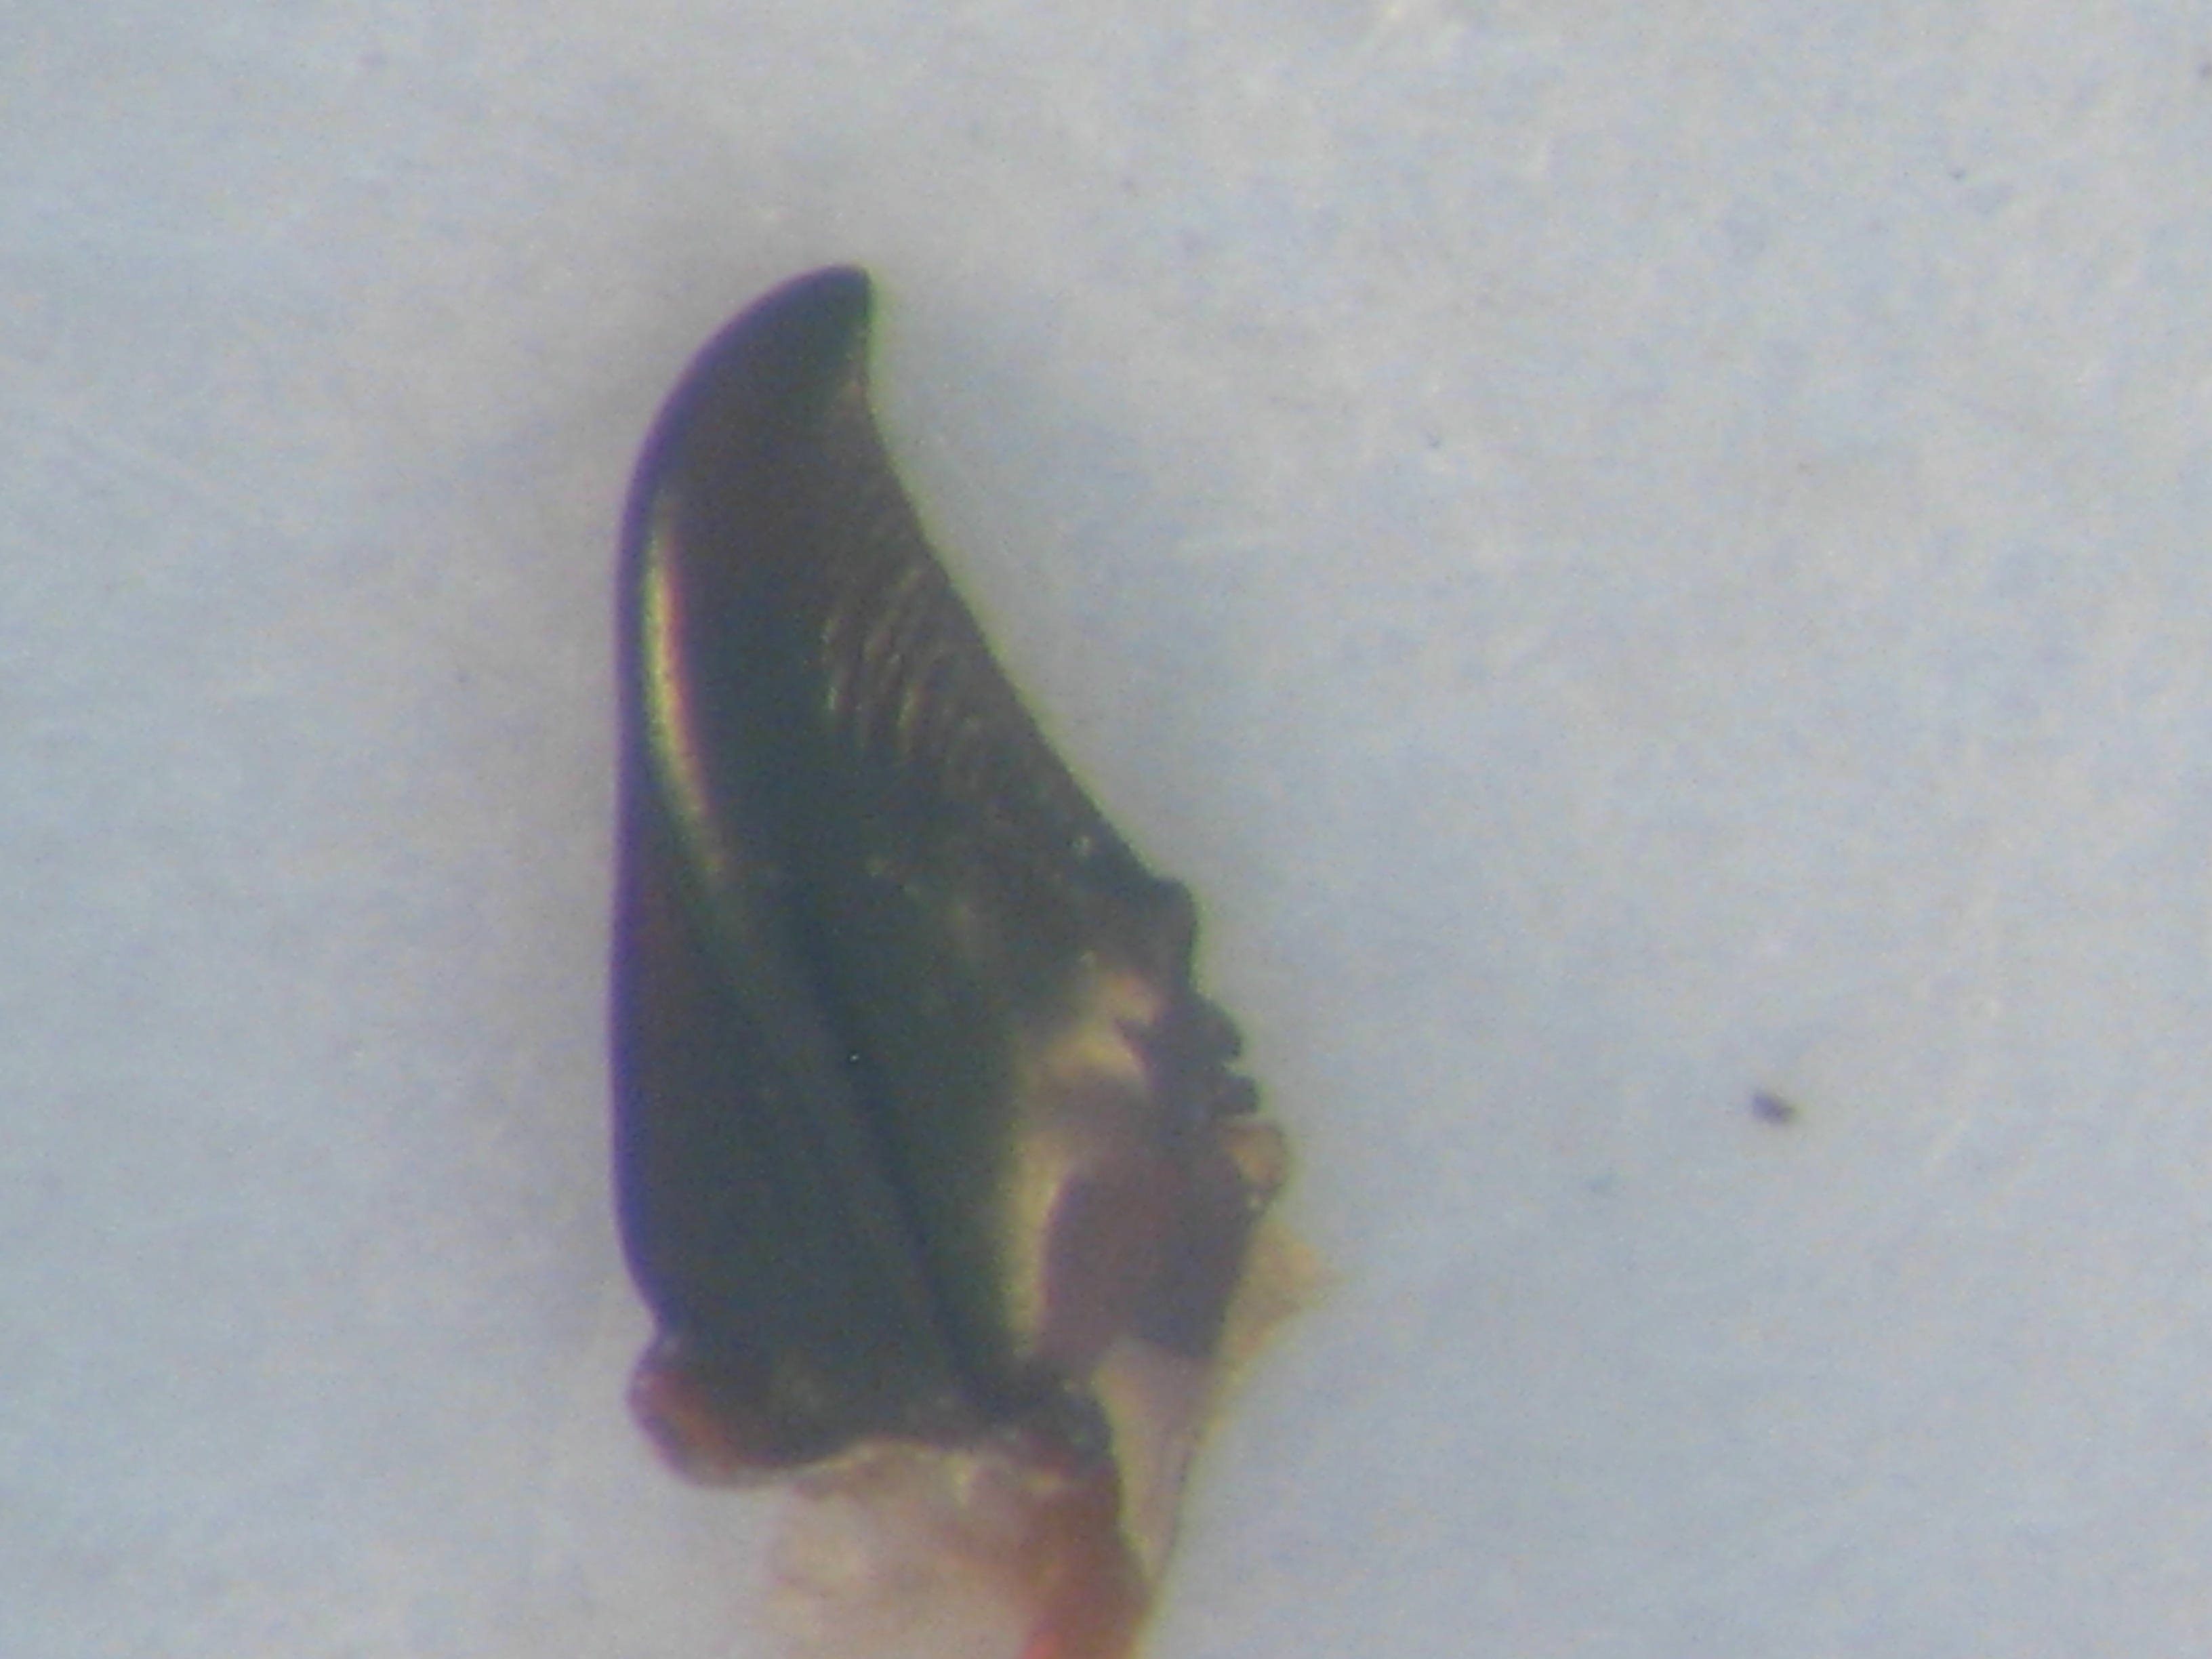
\includegraphics[width=0.22\textwidth]{./images/lm}}~~
\subfloat[Right mandible]{\label{figrbox1}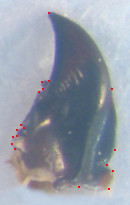
\includegraphics[width=0.22\textwidth]{./images/rm}}
\caption{The pictures of beetle mandibles took by biologists.}
\label{fig1}
\end{figure}

In recently, we have a lot of techniques to indicate the dominant points \cite{} but the applying them into morphometry analysis is limit in scope. In this paper, we focus on the method to automatically determine the landmarks in 2D biological images (see Fig. 1), specify beetle images. This method is a combination of principal component analysis (PCA) \cite{} and scale invariant feature transform (SIFT) \cite{•}. It includes three steps: (1) the contours of mandible shape are segment, (2) an iterative PCA is applied to register a source image and a target image and finally (3) the landmarks setting is done by using SIFT descriptor.
\section{Method}
For each beetle, the morphometric landmarks have been manually identified on mandibles images by the biologists: 16 and 18 landmarks for each left and right mandible, respectively. The consideration problem is how to detect automatically the landmarks on the mandible image to replace the manual ones. We propose a process includes three stages (1) segmentation, (2) registration, and (3) detection the landmarks. The Fig. \ref{fig2} shows the summary of the process. In the whole of the process, a source and a target image are used. The landmarks will be estimated on the target image by using the manual landmarks of the source image. Note, the source image is chosen randomly from the set of images.

\begin{figure}[htb]
    \centering
    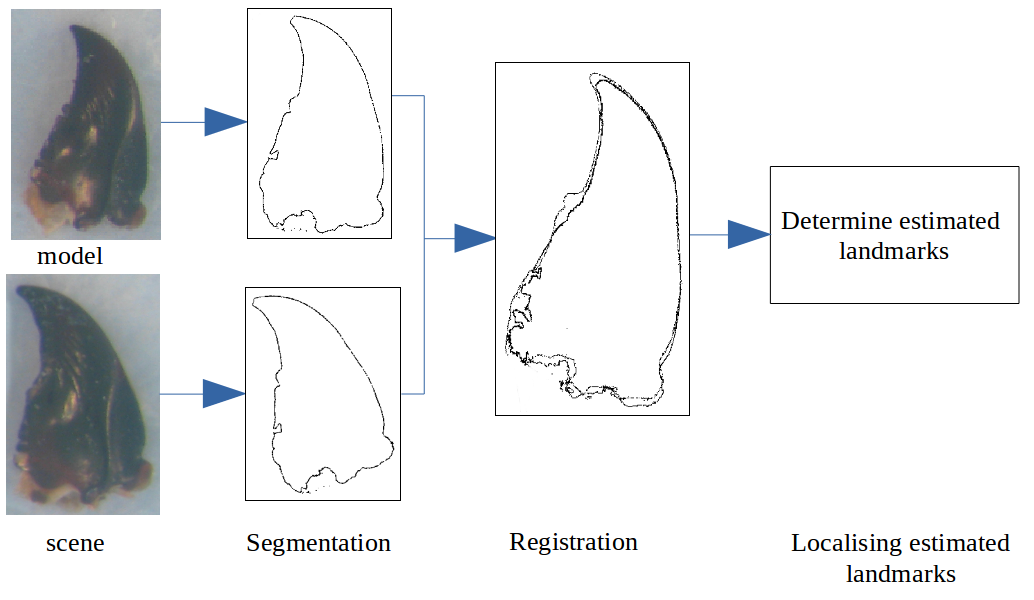
\includegraphics[width=0.5\textwidth]{./images/method}
    \caption{Overview of the proposed method}
    \label{fig2}
\end{figure}

In this section, firstly, we have a summary about the general utilization of SIFT. Then, we will discuss detail about our method with a difference way of SIFT to estimate the landmarks.
\subsection{SIFT method}
SIFT method proposed by Lowe\cite{} to extract distinctive invariant feature from images that can use to match between different views of source and target images such as rotation, scale, noise, 3D viewpoint. SIFT method includes four stages: (1) scale-space extrema detection, (2) keypoint localization, (3) orientation assignment, and (4) keypoint descriptor.

In the first stage, a difference of Gaussian (DoG) function is applied to identify the interest points on all scale and orientation of image. The key point candidates are localized and refined by suppress the key points which have the low contrast in the second stage. In the third stage, the orientation and gradient magnitude of key points are calculated. At the end, the descriptor is computed for each key point based on the orientation and gradient magnitude.

\begin{figure}[htb]
    \centering
    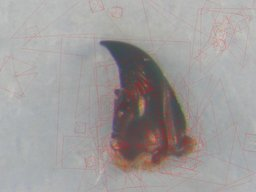
\includegraphics[width=0.3\textwidth]{./images/mdsift}
    \caption{SIFT keypoints in an right mandible}
    \label{fig3}
\end{figure}

By applying the original SIFT into our problem, we have succeeded indicating the keypoints in the image (see Fig. \ref{fig3}). But we do not have the result when we try to extract correspondence keypoints between the source and target image. The problem is carried from the choosing the best points from the large set of the candidates. This problem is solved in our method by limit the spatial before applied the SIFT along with changing the size of the grid to calculate the SIFT descriptor.
\subsection{Proposed method}
\subsubsection{Image segmentation}
\subsubsection{Image registration}
\subsubsection{Landmarks estimation}
\section{Experiments and result}
\section{Conclusion and discussion}
\subsection{\texttt{gretsi} class}
Your paper should not exceed 4 pages, including tables and
figures. It should consist of 2 columns each measuring 88mm wide,
with a gap of 6mm between the columns. We advise you to use the
\texttt{gretsi.cls} \LaTeXe\ class file to perform automatic page
setting:
\begin{verbatim}
    \documentclass{gretsi}
\end{verbatim}
In your file preamble, you have to enter the following informations:
\begin{itemize}

    \item paper title:\\
    \verb!\title{Paper title}!

    \item Christian and first names of each author, with a number
    linking to its address:\\
    \verb!\author{\coord{Pierre}{Dupont}{1},!\\
    \verb!        \coord{John}{Smith}{2}}!

    \item authors' addresses:\\
    \verb!\adresse{\affil{1}{Laboratory \\! \\
    \verb!         street, town, country}     ! \\
    \verb!         \affil{2}{University \\! \\
    \verb!         street, town, country}     !

    \item e-mail addresses:\\
    \verb!\email{First.Name@labo.fr, smith@univ.fr}!

    \item french and english written abstracts:\footnote{French
    written abstract is optional, but highly recommended.}\\
    \verb!\frenchabstract{R\'esum\'e fran\c{c}ais}! \\
    \verb!\englishabstract{English written abstract}!

    \item then, your text, and the bibliography: \\
    \verb!\begin{document}! \\
    \verb!\maketitle! \\
    \verb!Paper text! \\
    \verb!\begin{thebibliography}{99}! \\
    \verb!The references! \\
    \verb!\end{thebibliography}! \\
    \verb!\end{document}!

\end{itemize}

\subsection{Section and subsection}
This example file uses \verb!\section! and \verb!\subsection!. For
lower level sectioning commands, you obtain:
\subsubsection{Subsubsection}
By means of \verb!\subsubsection!.
\paragraph{Subsubsubsection}
By means of \verb!\paragraph!.

\section{Tables, figures and mathematics}
The title of tables should appear at the top, as in table
\ref{power}.
\begin{table}[htb]
    \caption{\label{power}2 to the power}
    \begin{center}
    \begin{tabular}{||c||*{8}{c|}|}
        \hline\hline
        $n$   & 1 & 2 & 3 &  4 &  5 &  6 &   7 &   8 \\ \hline
        $2^n$ & 2 & 4 & 8 & 16 & 32 & 64 & 128 & 256 \\
        \hline\hline
    \end{tabular}
    \end{center}
\end{table}

Captions should appear below graphical objects, as in figure \ref{circle}.
\begin{figure}[htb]
    \begin{center}
    \setlength{\unitlength}{0.5cm}
    \begin{picture}(5,5)
        \put(2.5,2.5){\oval(5,5)}
        \put(1,1){\line(1,0){3}}
        \put(4,1){\line(0,1){3}}
        \put(1,4){\line(1,0){3}}
        \put(1,1){\line(0,1){3}}
    \end{picture}
    \end{center}
    \caption{\label{circle}a square in an oval}
\end{figure}

Including \texttt{Postscript} graphics files is easily performed by
means of \texttt{graphics}, \texttt{graphicx} or \texttt{epsfig}
packages. To insert \texttt{fig.eps} file, with automatic width
adjustment, using \texttt{graphics} package, you have to enter:
\begin{verbatim}
    \begin{figure}[htb]
    \begin{center}
    \resizebox{88mm}{!}{
    \includegraphics{fig.eps}}
    \end{center}
    \legende{title}
    \end{figure}
\end{verbatim}
With \texttt{graphicx} package, you have to enter:
\begin{verbatim}
    \begin{figure}[htb]
    \begin{center}
    \includegraphics[width=88mm]{fig.eps}
    \end{center}
    \legende{title}
    \end{figure}
\end{verbatim}
With \texttt{epsfig}, you have to enter:
\begin{verbatim}
    \begin{figure}[htb]
    \begin{center}
    \epsfig{file=fig.eps,width=88mm}
    \end{center}
    \legende{title}
    \end{figure}
\end{verbatim}
Mathematical formulas appearence can be improved by means of
\texttt{amsmath} package from $\mathcal{AMS}$-\LaTeX. They
have to be numbered as formula \ref{formula}:
\begin{equation}
   \label{formula}
   F(x) = \int_{-\infty}^x f(u)\,du
\end{equation}

\begin{thebibliography}{99}

\bibitem{companion}
M.~Goossens, F~Mittelbach et A.~Samarin.
\emph{The \LaTeX{} Companion}.
Addison-Wesley, 1994.

\bibitem{lamport94a}
L.~Lamport.
\emph{\LaTeX{} User's Guide and Reference Manual}.
Addison-Wesley, 1994.

\end{thebibliography}

\end{document}
